\hypertarget{adding-new-instructions}{%
\chapter*{Adding New Instructions}\label{adding-new-instructions}}

\rightline{\textbf{{1 Week}}}

\section*{Motivation and introduction}

In this session, we will implement some custom instructions for an
application to speed up the execution time. Moreover, even when the
compiler uses the new instructions, they might not be used in all
optimization levels. For that, we will also introduce the feature, which
is used to add inline assembly to the application. By using inline
assembly, you can force the usage of custom instructions or you can
optimize bigger blocks (e.g. application hot spots) in hand written
assembler. For every part, that starts like ``a)'', ``b)'' \ldots{} you
have to mail the answers and asked files/tables to
\textbf{sajjad.hussain@kit.edu} and use the topic ``asipXX-Session4'',
with XX replaced by your group number.

\section*{Exercises}

\begin{enumerate}
\item \textbf{Preparing your project}
	\begin{enumerate}
		\item
		You can use the same project as in the last session, and just create
		a separate application subdirectory for each example. You can start
		a fresh project as in the Session 1, but this would be time
		consuming.
		\item
		For the C application, you have to create subdirectory in the
		``\emph{Application}'' directory (e.g. ``arrayloop''), and copy your
		application from ``\emph{/home/ces-asip00/Sessions/Session5/loop.c}'' to
		here.
		\item
		Copy a ``\emph{Makefile}'' file from the ``\emph{TestPrint}''
		application subdirectory to each application subdirectory.
		\item
		Set proper parameters and settings in ``\emph{env\_settings}.
		\item
		For these exercises, we will be using pipeline forwarding (-pf1)
		option which is the default one.
		\item
		Make sure that you already have VHDL files and GNU tools in your
		project's meister directory.
	\end{enumerate}
\item \textbf{Compiling and Simulating the Application}
	\begin{enumerate}
		\item
		First, you have to compile the application using gcc compiler to
		compare with the later results from dlxsim and ModelSim. To compile
		with GCC, comment the line ``\emph{\#define ASIP}'' and compile the
		application like ``\emph{gcc loop.c}''. For \emph{gcc} you can
		forward the printed output to a file, e.g. ``\emph{a.out
			\textgreater{} output\_gcc.txt}'' (`\emph{a.out}' is the default
		name of the binary that is created when you compile a program. The
		file `\emph{output\_gcc.txt}' will contain the printed array.
		\item
		Now, compile ``loop.c'' using ``make sim''. However, for compiling
		it, you first need to provide the required libraries, i.e.
		``\emph{lib\_lcd\_dlxsim''} (also for dlxsim/\emph{ModelSim}),
		``\emph{loadStoreByte''}, and ``\emph{string''}.
		\item
		After compiling, simulate the application in \emph{dlxsim} and
		\emph{ModelSim} and compare whether the printed results are the same
		compared to a \emph{gcc}-compiled version. The \emph{gcc} version
		will print the arrays on the screen and \emph{dlxsim} and
		\emph{ModelSim} will print them to a \emph{virtual} LCD. For
		\emph{dlxsim} you can forward the LCD output to a file, using the
		``\emph{-lf}'' parameter, e.g. ``\emph{make dlxsim
			DLXSIM\_PARAM=''-da0 --pf1 -lf\textbf{output\_dlxsim.txt}}'' writes
		output to the file ``\emph{output\_dsim.txt}''. \emph{ModelSim}
		automatically writes to the file ``\emph{lcd.out}''.
		\item
		To compare, whether the files generated from gcc, dlxsim \& ModelSim
		are identical, you can use command-line tools like ``\emph{diff
			output\_gcc.txt output\_ModelSim.txt}'' or graphical tools like
		``\emph{kompare}'' or ``\emph{kdiff3}''.
		\item
		Print statements should be commented out for a fair comparison. Then
		simulate in dlxsim and ModelSim.
		\begin{enumerate}[label=(\alph*)]
			\color{red}\item\normalcolor
			How many cycles do you need for execution in dlxsim and ModelSim
			(without printing)?
		\end{enumerate}
	\end{enumerate}
\item \textbf{Adding a new instruction to \emph{dlxsim Simulator}}
	\begin{enumerate}
		\def\labelenumii{\arabic{enumii}.}
		\item
		Create a project directory for this session by copying the directory
		``\emph{/home/ces-asip00/­epp/ASIP­Meister­Projects/TEMPLATE\_PROJECT/}''
		and renaming it (e.g. \emph{brownieAVG}).
		\item
		You have to create another subdirectory for our application in the
		``\emph{Application}'' directory (e.g. ``arrayloopAVG''). Copy
		``loop.c'' here and then you start putting new instructions here.
		Print statements should be comment out for a fair comparison.
		\item
		But before modifying ``loop.c'', create a simple C or assembly file
		to test different custom instruction (e.g. AVG) into an application
		subdirectory i.e. \emph{TestAVG}.
		\item
		Copy a ``\emph{Makefile}'' file from the ``\emph{TestPrint}''
		application subdirectory to each application subdirectory.
		\item
		Copy the provided \emph{ASIPMeister} CPU file
		``\emph{browstd32.pdb''} from ``/home/ces-asip00//Sessions/Session1/''
		into your project directory, and rename it
		``\emph{browstd32AVG.pdb''}
		\item
		Set proper parameters and settings in ``\emph{env\_settings}'' as
		discussed in Figure 2-5 in the Laboratory Script. Specially the
		followings:
\begin{lstlisting}
export PROJECT_NAME=brownieAVG
export CPU\_NAME=browstd32AVG
export ASIPMEISTER_PROJECTS_DIR=${HOME}/ASIPMeisterProjects
export DLXSIM_DIR=/home/ces-asip00/epp/dlxsimbr_Laboratory
\end{lstlisting}
	\item
	Now we start adding new instructions to our processor to speed up the
	execution. These new instructions are ``\emph{avg rd, rs0, rs1}'',
	``\emph{swap rd, rs}'', ``\emph{rot rd, rs0, amount}'' and
	``\emph{minmax rdMin, rdMax, rs0, rs1}''. First, implement the new
	instructions into \emph{dlxsim}, as explained in the Chapters 3.2.2
	and 3.2.3 of the Laboratory Script. Use the instruction format and
	opcodes as below:
\begin{lstlisting}
OpcodeInfo opcodes[] 	
//name	  class	                       op	mask	          other	flags	rangeMask
{"avg",        ARITH_3PARAM, 0x6c1,   0x1ffff, 	0x20, 	0 , 	0xffff8000 },
{"swap",     ARITH_2PARAM, 0x541,   0x1ffff, 	0x20, 	0 , 	0xffff8000 },
{"minmax", ARITH_4PARAM, 0x981,  0xfff, 		0x20, 	0 ,	0xffff8000 },
{"rot",	  ARITH_3PARAM,  0x8, 	 0x3f, 		0,  CHECK_LAST|IMMEDIATE_REQ, 0xffff8000 },
{"bgeu",     BRANCH_2OP, 0x11,   0x3f, 	0, 	0 , 	0 }***
*** Not needed in this session.
\end{lstlisting}
	\item
	Therefore, you have to copy \emph{dlxsim} to your local home (to be
	able to modify it) and you have to configure the
	``\emph{env\_settings''} to use your local \emph{dlxsim} (see Figure
	2-5 in the Laboratory Script).
		\begin{enumerate}[label=(\alph*),start=2]
		\color{red}\item\normalcolor
		Write a small assembly code to test your new instructions in dlxsim. You can use the Session2 assembly language program as the reference.
		\end{enumerate}
	\end{enumerate}
\item \textbf{Extending the CPU with a custom instruction}
	\begin{enumerate}
		\item
		In your new CPU, implement the new instruction ``\emph{avg rd, rs0,
			rs1}'', ``\emph{swap rd, rs}'', ``\emph{rot rd, rs amt}'' and
		``\emph{minmax rdMin, rdMax, rs0, rs1}'' as they are used in the
		application. This new instruction ``\emph{minmax}'' computes both
		the minimum and the maximum of two inputs \emph{rs0} and \emph{rs1}
		and write them simultaneously to two registers (\emph{rdMin} and
		\emph{rdMax}).
		\begin{quote}
		\textbf{Hint:}
		\end{quote}
	\begin{enumerate}
		\item
		You \textbf{can use the opcode and instruction formats as indicated in
			the figure below.}
		\item
		Do not implement the ``\emph{swap''} instruction as it is written in
		the C-code. Think what this instruction is doing and implement it
		without any shifts! Test the new instructions with a small assembly
		code in \emph{ModelSim}.
		\item
		For instructions that return two values, you need to change \# of GPR
		write ports. Normally, only one register is forwarded from EXE or WB
		stage, now you have to add new resources (Forwarding units) to forward
		two register values.
		\item
		Remember, that you cannot use a hardware resource twice in the same
		cycle, e.g. you cannot use the ALU twice in the EXE stage.
		Additionally, using it in two different pipeline stage significantly
		complicates the whole CPU design (just think about the required
		wiring).
		\item
		Remember that your new instruction has to support forwarding as well.
	\end{enumerate}
	\item
	Generate the VHDL Files.
	\item
	Please remember that for new custom instructions defined in
	ASIPmeister to be used automatically with C Compiler, you have to
	implement relevant ``\textbf{CKF Prototype}'' in ASIPmeister. Follow
	instructions at section 4.11.C in ASIPmeister tutorial and 11.2 in
	ASIPmeister user manual.
	\item
	Generate GNU Tools for your new processor.
\end{enumerate}
\item \textbf{Compiling and Simulating the Application with custom instructions}
	\begin{enumerate}
		\item
		You can test your custom instructions with small assembly programs.
		\item
		After testing the new instruction with a small assembly code, use
		\emph{inline assembly} in the application ``\emph{loop.c}'' for
		using the new instructions, see Chapter 8.2.3 in the Laboratory
		Script.
		\item
		There are two methods to insert a explicitly insert a custom
		instruction inside your C code:
		
		\begin{enumerate}
			\item
			Using \_\_builtin\_brownie32\_\_ABC directive: This method has a
			bug while using with the instruction that has zero return values
			or instructions that return more than one value. Examples:
\begin{lstlisting}
Int a,b,c,d;
c = __builtin_brownie32_AVG(a,b);
d = __builtin_brownie32_SWAP(a);
\end{lstlisting}
			\item	Using \_\_asm\_\_ directive: This can be used for all the cases.
\begin{lstlisting}
Branch Instruction
Int a,b,c,d,e;
__asm__ volatile (
"bgeu %[my_op1], %[my_op2], _here2\n"
"_there2: sub %[my_out], %[my_op1], %[my_op2]\n"
"_here2: add %[my_out], %[my_op1], %[my_op2]\n"
: [my_out] "=&r" (e)
: [my_op1] "r" (a),[my_op2] "r" (b)
);
__asm__ volatile (
"minmax %[my_out1], %[my_out2], %[my_op1], %[my_op2]\n\t"
: [my_out1] "=&r" (c), [my_out2] "=&r" (d)
: [my_op1] "r" (a), [my_op2] "r" (b)
);
\end{lstlisting}
	\end{enumerate}
	\item After modifying the application code by the \emph{inline assembly}
	stuffs for a particular custom instruction, compile the application
	using ``\emph{make sim}'', make sure that the result is still correct
	(\emph{diff} the \emph{ModelSim} output with gcc-compiled version) and
	find out, whether the new instructions have been used or not.

	\textbf{Note:} you have to check the generated assembly code to be sure
	that the new custom instructions are used in the code.
	\item
	Now you have to determine the number of cycles for executing the
	application to compute the speedup against the old CPU with the old
	compiler. {To determine the number of cycles you have to remove (i.e.
		comment out) the loop for printing the results}! Otherwise, this loop
	is the dominating hotspot and you will not notice a significant
	speedup when using the new assembly instructions!
	\item
	Simulate the application with ModelSim.
	\begin{enumerate}[label=(\alph*),start=3]
	\color{red}\item\normalcolor
	How many cycles do you need for execution in dlxsim and ModelSim?
	Attach assembly programs you used to test custom instructions with
	this mail.
	\color{red}\item\normalcolor
	What is the speedup (i.e. \#Cycles without custom instructions /
	\#Cycles with custom instructions)?
	\color{red}\item\normalcolor
	Attach the assembly and/or C file you used to test the custom
	instruction and to test the given application.
	\color{red}\item\normalcolor
	Attach the modified ASIPmeister.pdb file.
	\end{enumerate}
	\end{enumerate}
\end{enumerate}
%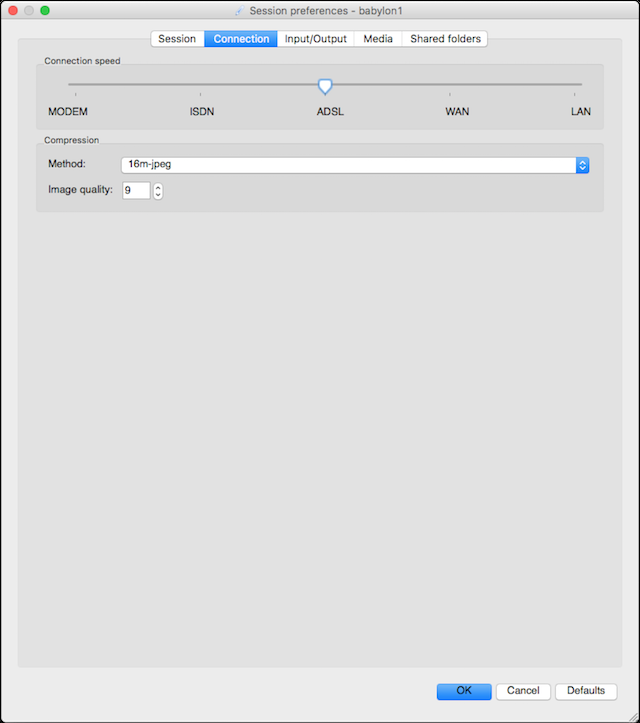
\includegraphics[width=6.4054in,height=5.31336in]{media/image2.png}

\textbf{Next Session:} Bubble Sort -- Simulations and Optimization

\textbf{Readings for the next session}: All the Chapters, especially 4
\& 8, ASIPMeister Tutorial \& Manual

\begin{figure}
	\centering
	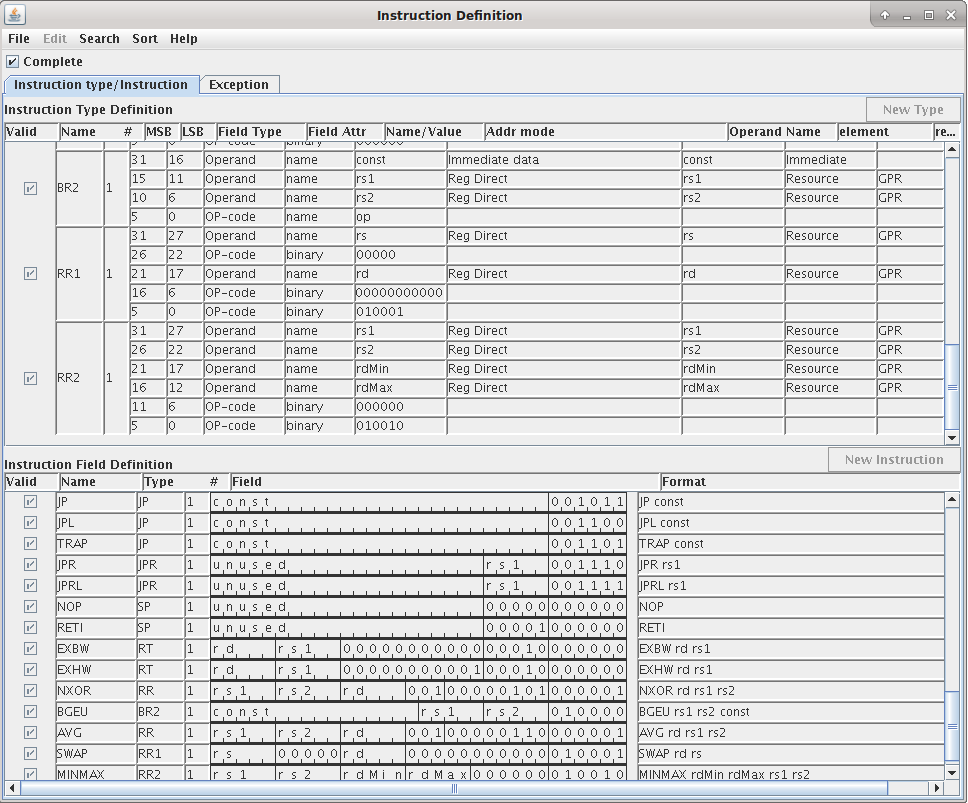
\includegraphics[width=0.9\textwidth]{src/images/image1.png}
	\caption{Instruction Definitions and OpCodes}
	\label{fig:fig1}
\end{figure}